% Created 2021-07-26 Mon 11:04
% Intended LaTeX compiler: pdflatex
\documentclass[presentation,aspectratio=1610]{beamer}
\usepackage[utf8]{inputenc}
\usepackage[T1]{fontenc}
\usepackage{graphicx}
\usepackage{grffile}
\usepackage{longtable}
\usepackage{wrapfig}
\usepackage{rotating}
\usepackage[normalem]{ulem}
\usepackage{amsmath}
\usepackage{textcomp}
\usepackage{amssymb}
\usepackage{capt-of}
\usepackage{hyperref}
\usepackage{khpreamble, euscript}
\DeclareMathOperator{\atantwo}{atan2}
\newcommand*{\ctrb}{\EuScript{C}}
\newcommand*{\obsv}{\EuScript{O}}
\usetheme{default}
\author{Kjartan Halvorsen}
\date{\today}
\title{Output feedback (observer)}
\hypersetup{
 pdfauthor={Kjartan Halvorsen},
 pdftitle={Output feedback (observer)},
 pdfkeywords={},
 pdfsubject={},
 pdfcreator={Emacs 26.3 (Org mode 9.4.6)}, 
 pdflang={English}}
\begin{document}

\maketitle

\section{Apollo moon lander}
\label{sec:orgf367148}
\begin{frame}[label={sec:orga00b35e}]{Example - The Apollo lunar module}
\begin{center}
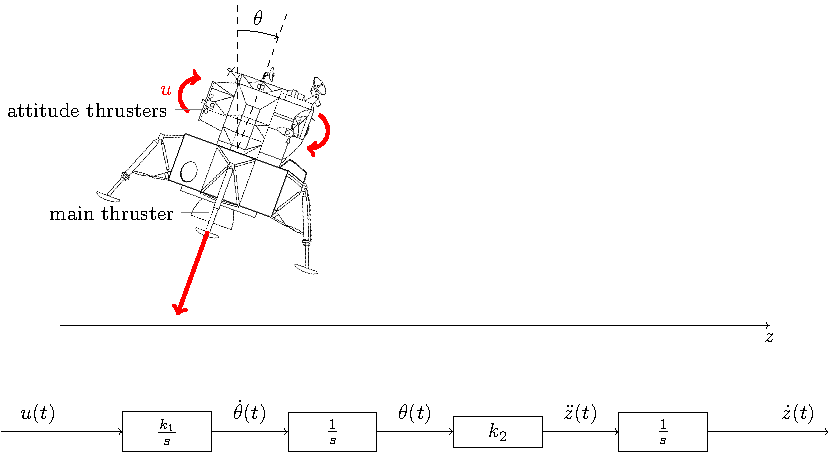
\includegraphics[width=\linewidth]{fig-apollo}
\end{center}
\end{frame}

\begin{frame}[label={sec:org4e808de}]{Example - The Apollo lunar module}
State variables: \(x = \begin{bmatrix} x_1 & x_2 & x_3 \end{bmatrix}^T = \begin{bmatrix} \dot{\theta} & \theta & \dot{z} \end{bmatrix}^T\). With dynamics
\[ \begin{cases} \dot{x}_1 =  \ddot{\theta} = k_1 u\\ \dot{x}_2 = \dot{\theta} = x_1\\ \dot{x}_3 = \ddot{z} = k_2\theta = k_2x_2 \end{cases} \]

\[ \dot{x} = \begin{bmatrix} \dot{x}_1\\\dot{x}_2\\\dot{x}_3\end{bmatrix} = \underbrace{\begin{bmatrix} \textcolor{red!60!black}{0} & \textcolor{red!60!black}{0} &\textcolor{red!60!black}{0} \\\textcolor{red!60!black}{1} & \textcolor{red!60!black}{0}& \textcolor{red!60!black}{0}\\ \textcolor{red!60!black}{0}& \textcolor{red!60!black}{k_2} &\textcolor{red!60!black}{0} \end{bmatrix}}_{A} \begin{bmatrix} x_1\\x_2\\x_3\end{bmatrix} + \underbrace{\begin{bmatrix} \textcolor{red!60!black}{k_1} \\ \textcolor{red!60!black}{0} \\\textcolor{red!60!black}{0}  \end{bmatrix}}_{B} u \]
\end{frame}


\begin{frame}[label={sec:org03fd31b}]{Example - The Apollo lunar module}
 \begin{align*}
  x(kh+h) &= \mathrm{e}^{Ah} x(kh) + \int_{0}^{h} \mathrm{e}^{As} B u(kh+h-s) ds\\
   &= \underbrace{\mathrm{e}^{Ah}}_{\Phi(h)} x(kh) + \underbrace{\left(\int_{0}^h \mathrm{e}^{As} B ds \right)}_{\Gamma(h)} u(kh)\\
   &= \begin{bmatrix} 1 & 0 & 0\\h & 1 & 0\\\frac{h^2k_2}{2} & hk_2 & 1\end{bmatrix} x(kh) + k_1 \begin{bmatrix} h\\ \frac{h^2}{2} \\ \frac{k_2 h^3}{6} \end{bmatrix} u(kh)
\end{align*}
\end{frame}


\section{State feedback with observer}
\label{sec:org1049069}
\begin{frame}[label={sec:orge0b900b}]{State feedback with reconstructed states}
\end{frame}

\begin{frame}[label={sec:org7f98d83}]{State feedback with reconstructed states}
\begin{center}
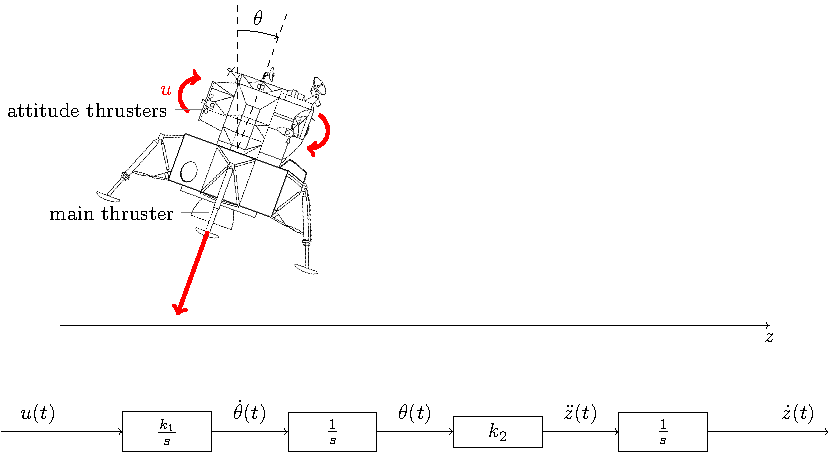
\includegraphics[width=0.9\linewidth]{fig-apollo}
\end{center}
\end{frame}

\begin{frame}[label={sec:org5b63c86}]{State feedback}
Given
 \begin{equation}
 \begin{split}
  x(k+1) &= \Phi x(k) + \Gamma u(k)\\
  y(k) &= C x(k)
 \end{split}
 \label{eq:ssmodel}
\end{equation}
and measurements (or estimates) of the state vector \(x(k)\). 

\alert{Linear state feedback} is the control law
\begin{equation*}
\begin{split}
 u(k) &= f\big((x(k), u_c(k)\big) = -l_1x_1(k) - l_2x_2(k) - \cdots - l_n x_n(k) + l_0u_c(k)\\
      &= -Lx(k) + l_0u_c(k), 
\end{split}
\end{equation*}
where \[ L = \bbm l_1 & l_2 & \cdots & l_n \ebm. \]
Substituting the control law in the state space model \eqref{eq:ssmodel} gives
 \begin{equation}
 \begin{split}
  x(k+1) &= \left(\Phi -\Gamma L \right) x(k) + l_0\Gamma u_c(k)\\
  y(k) &= C x(k)
 \end{split}
 \label{eq:closedloop}
\end{equation}
\end{frame}



\begin{frame}[label={sec:org71af002}]{Observer design}
Given model
 \begin{equation*}
 \begin{split}
  x(k+1) &= \Phi x(k) + \Gamma u(k)\\
  y(k) &= C x(k)
 \end{split}
 \label{eq:ssmodel}
\end{equation*}
and measurements of the output signal \(y(k)\). 

The obserser is given by
\begin{equation*}
\begin{split}
\hat{x}(k+1) &= \underbrace{\Phi \hat{x}(k) + \Gamma u(k)}_{\text{simulation}} + \underbrace{K\big(y(k) - C\hat{x}(k)\big)}_{\text{correction}} = \left(\Phi - KC\right)\hat{x}(k) +  \Gamma u(k) + Ky(k)
\end{split}
\end{equation*}
with poles given by the eigenvalues of the matrix \(\Phi_o = \Phi - KC\)

\alert{Rule-of-thumb} Choose the poles of the observer (eigenvalues of \(\Phi-KC\)) at least twice as fast as the poles (eigenvalues) of \(\Phi-\Gamma L\).
\end{frame}

\begin{frame}[label={sec:org8c2ca3d}]{Observer design}
\alert{Rule-of-thumb} Choose the poles of the observer (eigenvalues of \(\Phi-KC\)) at least twice as fast as the poles (eigenvalues) of \(\Phi-\Gamma L\).

In continuous time (the s-plane), choosing a pole to be twice as fast, means moving the pole to twice the disance from the origin. Given a discrete pole \(p_1\), the discrete pole in 
\[ p_2 = \text{exp}\left( 2 \frac{\ln p_1}{h} h\right) = \text{exp} \big( 2 \ln p_1 \big) = p_1^2\]
corresponds to a response that is twice as fast.
\end{frame}

\begin{frame}[label={sec:org71f4946}]{Control by feedback from reconstructed states}
The design problem can be separates into two problems
\begin{enumerate}
\item Determine the gain vector \(\textcolor{orange!80!black}{L}\) and the gain \(l_0\) of the control law
\[ u(k) = -\textcolor{orange!80!black}{L} \hat{x}(k) + l_0 u_c(k)\]
so that the closed-loop system has good reference tracking.
\item Determine the gain vector \(\textcolor{red}{K}\) of the observer
\begin{equation*}
\begin{split}
\hat{x}(k+1) &= \Phi \hat{x}(k) + \Gamma u(k) + \textcolor{red}{K} \big(y(k) - C\hat{x}(k)\big)
\end{split}
\end{equation*}
to get a good balance between disturbance rejection and noise attenuation.
\end{enumerate}
\end{frame}

\begin{frame}[label={sec:orgff3fa4d}]{Computing the observer gain}
A matrix \(M\) and its transpose \(M\transp\) have the same eigenvalues. Hence, the problem of determining the gain \(K\) to obtain desired eigenvalues of 
\[\Phi- KC\] is equivalent to determining the gain \(K\) in 
\[(\Phi-KC)\transp = \Phi\transp - C\transp K\transp.\]
The last problem has the exact same form as the problem of determining \(L\) to obtain desired eigenvalues of 
\[\Phi - \Gamma L\]

So, the same matlab function can be used for both problems.
\end{frame}

\begin{frame}[label={sec:org9d34dd5},fragile]{Computing the observer gain}
 \begin{enumerate}
\item \alert{Ackerman's method} 
\begin{verbatim}
K = acker(Phi', C', po)'
\end{verbatim}
\item \alert{More numerically stable method} 
\begin{verbatim}
K = place(Phi', C', pd)'
\end{verbatim}
\end{enumerate}
\end{frame}
\end{document}